\documentclass[12pt]{article} %set font size and document type
\usepackage{graphicx} % Required for inserting images
\usepackage[useregional]{datetime2} %allow use of \today
\usepackage[margin=1in]{geometry} % set margins
\usepackage{setspace} % allow setting of double and single spacing
\usepackage{hyperref} % creates clickable table of contents
\usepackage{adjustbox} % allows us to rotate images, tables, etc.
\usepackage{capt-of}  % dwb added

% \usepackage{xcolor}
\usepackage{color, colortbl}

\usepackage{listings}
\newcommand{\lsin}[1]{\lstinline[columns=fullflexible,keepspaces=true,language=Java,basicstyle=\footnotesize\ttfamily]{#1}}

\lstdefinelanguage{Java}{
  columns=fullflexible,keepspaces=true,basicstyle=\scriptsize\ttfamily,
%  basicstyle=\scriptsize\sffamily,
  numbers=left,
  xleftmargin=5.0ex,
  escapechar=@,
  sensitive=true,
  otherkeywords={},
  morekeywords=[1]{int,while,if,public,static,else,return,new,for,return,void},
  keywordstyle={[1]\bfseries\color{blue}},
  numberstyle=\tiny\color{black},
  rulecolor=\color{black},
}

% set up header and footer
\usepackage{titleps,kantlipsum}
\newpagestyle{mypage}{%
  \headrule
  \sethead{\MakeUppercase{\thesection\quad \sectiontitle}}{}{\thesubsection\quad \subsectiontitle}
  \setfoot{}{}{\em{p. \thepage}}
}
\settitlemarks{section,subsection}
\pagestyle{mypage}

% set up title information 
% Students replace project title and their names here
\title{War Online
\\
CS482 Software Engineering}
\author{Jonathan Ramos, Ayoposi Olu-Bamisaye, Brett Bonner\\
Client: Dr. Eric Cui}
\date{\today}

\begin{document}

\maketitle

% creates table of contents
\pagebreak
\tableofcontents
\section*{Abstract}



%[[ text between `[[' and `]]' are comments from me to you and should be
%commented out as you complete various section 

%Put here the \emph{elevator pitch} for your project. 

%IOW a 1-2 paragraph summary of your project
%that includes who the client is and why they need this App.]]

Our project is focused on developing a web app for Dr. Cui and his company, Cosmic Radiance, to implement an engaging online card game. Cosmic Radiance aims to attract and retain users by offering an interactive and immersive experience through this game. The app will provide features that encourage regular play and a user-friendly interface to enhance engagement. By leveraging an online format, the card game will allow Cosmic Radiance to build a loyal user base, supporting the company’s goal of fostering a vibrant community and increasing user retention overall.





\pagebreak
% make body of document double spaced for easier feedback writing
% \doublespacing 


% include the latex files with the content
\section{Introduction}

%[[ No more than one page that provides a short project description and then
%sets the stage for the rest of the document. ]]

%This sentence has an example citation~\cite{DBLP:journals/infsof/BinkleyMI22}

In today's increasingly rapid changing digital world, keeping users engaged is essential to making interactive applications successful. To keep users engaged, they must feel connected and entertained. Our client seeks to develop an engaging, real-time multiplayer card game, to engage users and improve long-term user retention. The application overall should provide compelling game play experience with social interaction and an easy to understand user interface. 


To address our clients needs, we proposed an extensive software solution that leverages modern web development technologies. The application features a responsive and dynamic front end built using HTML, CSS, and JavaScript with React. React's component based architecture allows us to create reusable modules that ensures consistency and streamlines development as each component can be developed independently. All of the React components we build return HTML that can be dynamically injected into our main HTML file. The program logic is handled appropriately depending on the purpose the code serves. Each component handles its necessary back-end logic locally and at the end returns the necessary HTML for the front-end.  Non-react component files do not return any HTML for the front-end such as the JavaScript Class that establishes the deck and card structures. Additionally, by using Firebase, we ensure real time data synchronization and built-in authentication, both necessary for a seamless multiplayer experience. 


Key features our application include, Real-Time Gameplay, Engaging user Experience, User Authentication, and Social Interaction. Each of these features is necessary to delivering an immersive experience for the users. Real-Time Gameplay ensures all players at a game table receive the same instant updates and feedback, crucial for maintaining the flow of the game. An engaging user experience includes a visually appealing, intuitive, and responsive interface, all necessary to retaining users. The front end is built using HTML, CSS, JavaScript and React, which allows us to create a highly dynamic user interface. The inclusion of user authentication is necessary to allow for socialization and a friend system in the application. As multiplayer games rely on social interaction, our application includes features that encourage social interactions between players through the friends and chats system.


This document serves a detailed roadmap for the development of the multiplayer card game War for our client Cosmic Radiance. It starts by outlining the requirements of the software to identify the needs of the application. Additionally, this section will provide an overview of the different requirements of each user type. The following section provides a detailed look at each Iteration (sprint) of the project. Each iteration subsection will cover the proposed plan for the sprint, activities, testing, and a retrospective. The System Architecture and Design section focuses on the design considerations that influenced the project's chosen technologies. The Testing section focuses on the testing process throughout the development of the application, as well as the overall coverage. 
 
 
  





\section{Requirements}


\subsection{User Roles}

%[[ Describe the types of users of your App.
%What is their technical expertise, what security level access should they have,
%etc.
%The purpose of this list is to help you ensure you are meeting the clients
%needs in your requirements.
%The names you use here to describe roles should match what you use in your
%user stories and \emph{reflect the clients vocabulary.}

Our application consists of three types of users, Player, Host, and Admin. 


\subsubsection{Player}
The player should have access to all profile, friend, and chat functionalities.
Player is also able to join a table and play the round, however, they are not able to deal cards as only the host of the table should be able to start the game by dealing the cards. 

\subsubsection{Host}
The Host should have access to all functionalities of a Player. However, a host creates new tables for other Players to join. Additionally, the host is also able to start the game by dealing the cards once another Player connects to the Host's table. 

\subsubsection{Admin}
The Admin should have access to all user's information. An admin can modify user information as needed, they should be able to reset a user's password, or update their username. An admin should also be able to completely remove and create accounts as needed. 


\subsection{Functional Requirement User Stories and Tasks}



\subsubsection{Player}

\textbf{S1: Create User (2)}
\begin{enumerate}
    \item Priority: High
    \item \textbf{I want} to create an account
    \item \textbf{So that} I can play the game
    \item \textbf{Definition of Done:} When I am able to create a new account
    \item \textbf{Depends On:} N/A
    \item Tasks: N/A
    %\begin{enumerate}
    % For each task write the ID, :, then title. Then describe the task.
        %\item Task [[ ID: Title. Description.]]
    %\end{enumerate}
\end{enumerate}


\textbf{S2: Guest Account (1)}
\begin{enumerate}
    \item Priority: High
    \item \textbf{I want} to play as a guest
    \item \textbf{So that} I can play without registering
    \item \textbf{Definition of Done:} When I am able to play without registering
    \item \textbf{Depends On:} N/A
    \item Tasks: N/A
    %\begin{enumerate}
    % For each task write the ID, :, then title. Then describe the task.
        %\item Task [[ ID: Title. Description.]]
    %\end{enumerate}
\end{enumerate}


\textbf{S3: Login (1)}
\begin{enumerate}
    \item Priority: High
    \item \textbf{I want} to log in to my account
    \item \textbf{So that} I can play access my saved data
    \item \textbf{Definition of Done:} When I am able to access my previously created account
    \item \textbf{Depends On:} S2: Create Account
    \item Tasks: N/A
    %\begin{enumerate}
    % For each task write the ID, :, then title. Then describe the task.
        %\item Task [[ ID: Title. Description.]]
    %\end{enumerate}
\end{enumerate}


\textbf{S4: Logout (1)}
\begin{enumerate}
    \item Priority: High
    \item \textbf{I want} to log out of my account
    \item \textbf{So that} only I have access to my account
    \item \textbf{Definition of Done:} When I am able to control access to my account
    \item \textbf{Depends On:} S3: Login
    \item Tasks: N/A
    %\begin{enumerate}
    % For each task write the ID, :, then title. Then describe the task.
        %\item Task [[ ID: Title. Description.]]
    %\end{enumerate}
\end{enumerate}


\textbf{S5: Password (2)}
\begin{enumerate}
    \item Priority: High
    \item \textbf{I want} to change my password
    \item \textbf{So that} I can secure my account
    \item \textbf{Definition of Done:} When I am able to secure my account
    \item \textbf{Depends On:} N/A
    \item Tasks: N/A
    %\begin{enumerate}
    % For each task write the ID, :, then title. Then describe the task.
        %\item Task [[ ID: Title. Description.]]
    %\end{enumerate}
\end{enumerate}


\textbf{S6: Update (1)}
\begin{enumerate}
    \item Priority: Medium
    \item \textbf{I want} to update personal information
    \item \textbf{So that} I have an accurate profile
    \item \textbf{Definition of Done:} When I am able to update my account
    \item \textbf{Depends On:} N/A
    \item Tasks: N/A
    %\begin{enumerate}
    % For each task write the ID, :, then title. Then describe the task.
        %\item Task [[ ID: Title. Description.]]
    %\end{enumerate}
\end{enumerate}


\textbf{S7: Profile Avatar (2)}
\begin{enumerate}
    \item Priority: Medium
    \item \textbf{I want} to add a profile picture
    \item \textbf{So that} I can show off my creativity
    \item \textbf{Definition of Done:} When I am able to choose a profile picture
    \item \textbf{Depends On:} N/A
    \item Tasks: N/A
    %\begin{enumerate}
    % For each task write the ID, :, then title. Then describe the task.
        %\item Task [[ ID: Title. Description.]]
    %\end{enumerate}
\end{enumerate}


\textbf{S8: Add Friend (2)}
\begin{enumerate}
    \item Priority: High
    \item \textbf{I want} to add another player as a friend
    \item \textbf{So that} I can easily connect with friends
    \item \textbf{Definition of Done:} When I am able to add another player to my list of friends
    \item \textbf{Depends On:} N/A
    \item Tasks: N/A
    %\begin{enumerate}
    % For each task write the ID, :, then title. Then describe the task.
        %\item Task [[ ID: Title. Description.]]
    %\end{enumerate}
\end{enumerate}


\textbf{S9: Remove Friend (2)}
\begin{enumerate}
    \item Priority: High
    \item \textbf{I want} to remove another player as a friend
    \item \textbf{So that} I can shorten my friends list
    \item \textbf{Definition of Done:} When I am able to remove another player from my list of friends
    \item \textbf{Depends On:} N/A
    \item Tasks: N/A
    %\begin{enumerate}
    % For each task write the ID, :, then title. Then describe the task.
        %\item Task [[ ID: Title. Description.]]
    %\end{enumerate}
\end{enumerate}


\textbf{S10: Show Friends (1)}
\begin{enumerate}
    \item Priority: High
    \item \textbf{I want} to see my list of friends
    \item \textbf{So that} I know who my friends are
    \item \textbf{Definition of Done:} When I am able to see all the players in my friends list
    \item \textbf{Depends On:} S8: Add Friend 
    \item Tasks: N/A
    %\begin{enumerate}
    % For each task write the ID, :, then title. Then describe the task.
        %\item Task [[ ID: Title. Description.]]
    %\end{enumerate}
\end{enumerate}


\textbf{S11: Invite Friend (3)}
\begin{enumerate}
    \item Priority: High
    \item \textbf{I want} to invite a friend to my table
    \item \textbf{So that} I can play at the same table as my friend
    \item \textbf{Definition of Done:} When I am able to invite another player to my table
    \item \textbf{Depends On:} N/A
    \item Tasks: N/A
    %\begin{enumerate}
    % For each task write the ID, :, then title. Then describe the task.
        %\item Task [[ ID: Title. Description.]]
    %\end{enumerate}
\end{enumerate}


\textbf{S12: Display Stats (1)}
\begin{enumerate}
    \item Priority: Low
    \item \textbf{I want} to show off my stats (W/L)
    \item \textbf{So that} I can compare with my friends
    \item \textbf{Definition of Done:} When I can compare stats
    \item \textbf{Depends On:} N/A
    \item Tasks: N/A
    %\begin{enumerate}
    % For each task write the ID, :, then title. Then describe the task.
        %\item Task [[ ID: Title. Description.]]
    %\end{enumerate}
\end{enumerate}


\textbf{S13: Report Player (2)}
\begin{enumerate}
    \item Priority: Medium
    \item \textbf{I want} to report another player for violations
    \item \textbf{So that} I can ensure players are following rules/guidelines
    \item \textbf{Definition of Done:} When I am able to report a player
    \item \textbf{Depends On:} N/A
    \item Tasks: N/A
    %\begin{enumerate}
    % For each task write the ID, :, then title. Then describe the task.
        %\item Task [[ ID: Title. Description.]]
    %\end{enumerate}
\end{enumerate}


\textbf{S14: Public Chat (3)}
\begin{enumerate}
    \item Priority: High
    \item \textbf{I want} to send messages to the entire table
    \item \textbf{So that} I can communicate publicly
    \item \textbf{Definition of Done:} I can communicate with the table
    \item \textbf{Depends On:} N/A
    \item Tasks: N/A
    %\begin{enumerate}
    % For each task write the ID, :, then title. Then describe the task.
        %\item Task [[ ID: Title. Description.]]
    %\end{enumerate}
\end{enumerate}


\textbf{S15: Private Chat (3)}
\begin{enumerate}
    \item Priority: High
    \item \textbf{I want} to send messages to my friends
    \item \textbf{So that} I can communicate outside of table-chat (public chat)
    \item \textbf{Definition of Done:} I can communicate privately
    \item \textbf{Depends On:} N/A
    \item Tasks: N/A
    %\begin{enumerate}
    % For each task write the ID, :, then title. Then describe the task.
        %\item Task [[ ID: Title. Description.]]
    %\end{enumerate}
\end{enumerate}


\textbf{S16: Review Chat (2)}
\begin{enumerate}
    \item Priority: Low
    \item \textbf{I want} to view previous messages
    \item \textbf{So that} I can review my conversations
    \item \textbf{Definition of Done:} Private chats are saved
    \item \textbf{Depends On:} S15: Private Chat
    \item Tasks: N/A
    %\begin{enumerate}
    % For each task write the ID, :, then title. Then describe the task.
        %\item Task [[ ID: Title. Description.]]
    %\end{enumerate}
\end{enumerate}


\textbf{S17: Lobby (5)}
\begin{enumerate}
    \item Priority: High
    \item \textbf{I want} to access the lobby 
    \item \textbf{So that} I can see live tables, see open/closed tables, sort by amount of tables
    \item \textbf{Definition of Done:} I am able to access the lobby correctly
    \item \textbf{Depends On:} N/A
    \item Tasks: N/A
    %\begin{enumerate}
    % For each task write the ID, :, then title. Then describe the task.
        %\item Task [[ ID: Title. Description.]]
    %\end{enumerate}
\end{enumerate}


\textbf{S18: Tutorial (3)}
\begin{enumerate}
    \item Priority: High
    \item \textbf{I want} the ability to do the tutorial 
    \item \textbf{So that} I can learn to play the game
    \item \textbf{Definition of Done:} Players understand the game
    \item \textbf{Depends On:} N/A
    \item Tasks: N/A
    %\begin{enumerate}
    % For each task write the ID, :, then title. Then describe the task.
        %\item Task [[ ID: Title. Description.]]
    %\end{enumerate}
\end{enumerate}


\textbf{S19: Table (5)}
\begin{enumerate}
    \item Priority: High
    \item \textbf{I want} to start my own table 
    \item \textbf{So that} I can play with friends or random people
    \item \textbf{Definition of Done:} My friends or random people can join my table
    \item \textbf{Depends On:} N/A
    \item Tasks: N/A
    %\begin{enumerate}
    % For each task write the ID, :, then title. Then describe the task.
        %\item Task [[ ID: Title. Description.]]
    %\end{enumerate}
\end{enumerate}


\textbf{S20: Currency (1)}
\begin{enumerate}
    \item Priority: Medium
    \item \textbf{I want} to raise the stakes of my table
    \item \textbf{So that} I can make more "fake" currency
    \item \textbf{Definition of Done:} I can set the currency for my table
    \item \textbf{Depends On:} N/A
    \item Tasks: N/A
    %\begin{enumerate}
    % For each task write the ID, :, then title. Then describe the task.
        %\item Task [[ ID: Title. Description.]]
    %\end{enumerate}
\end{enumerate}


\textbf{S22: Bot (5)}
\begin{enumerate}
    \item Priority: Medium
    \item \textbf{I want} to play with a bot
    \item \textbf{So that} I can play without friends
    \item \textbf{Definition of Done:} When a bot plays the game with the player
    \item \textbf{Depends On:} N/A
    \item Tasks: N/A
    %\begin{enumerate}
    % For each task write the ID, :, then title. Then describe the task.
        %\item Task [[ ID: Title. Description.]]
    %\end{enumerate}
\end{enumerate}



\subsubsection{Host}

\textbf{S21: Start Game (3)}
\begin{enumerate}
    \item Priority: High
    \item \textbf{I want} to start the game
    \item \textbf{So that} I can play the game
    \item \textbf{Definition of Done:} When I am able to successfully start the game
    \item \textbf{Depends On:} N/A
    \item Tasks: N/A
    %\begin{enumerate}
    % For each task write the ID, :, then title. Then describe the task.
        %\item Task [[ ID: Title. Description.]]
    %\end{enumerate}
\end{enumerate}


\subsubsection{Admin}

\textbf{S23: Manage Users (1)}
\begin{enumerate}
    \item Priority: High
    \item \textbf{I want} to view a list of all registered users
    \item \textbf{So that} I can monitor and manage all users
    \item \textbf{Definition of Done:} When I can display all registered users in the system
    \item \textbf{Depends On:} S1: Create User
    \item Tasks: N/A
    %\begin{enumerate}
    % For each task write the ID, :, then title. Then describe the task.
        %\item Task [[ ID: Title. Description.]]
    %\end{enumerate}
\end{enumerate}


\textbf{S24: Manage Tables (3)}
\begin{enumerate}
    \item Priority: Medium
    \item \textbf{I want} to monitor games in real-time
    \item \textbf{So that} I can ensure proper gameplay
    \item \textbf{Definition of Done:} When I can interact with tables in real-time
    \item \textbf{Depends On:} S19: Table
    \item Tasks: N/A
    %\begin{enumerate}
    % For each task write the ID, :, then title. Then describe the task.
        %\item Task [[ ID: Title. Description.]]
    %\end{enumerate}
\end{enumerate}


\textbf{S25: Manage Ads (3)}
\begin{enumerate}
    \item Priority: High
    \item \textbf{I want} to create and manage ads
    \item \textbf{So that} I can make money and promote my company
    \item \textbf{Definition of Done:} When I can add and delete different ads on the website
    \item \textbf{Depends On:} N/A
    \item Tasks: N/A
    %\begin{enumerate}
    % For each task write the ID, :, then title. Then describe the task.
        %\item Task [[ ID: Title. Description.]]
    %\end{enumerate}
\end{enumerate}


\textbf{S26: Analytics (1)}
\begin{enumerate}
    \item Priority: Medium
    \item \textbf{I want} to track player data
    \item \textbf{So that} I can analyze the app's growth
    \item \textbf{Definition of Done:} When I can view information on the app's performance
    \item \textbf{Depends On:} N/A
    \item Tasks: N/A
    %\begin{enumerate}
    % For each task write the ID, :, then title. Then describe the task.
        %\item Task [[ ID: Title. Description.]]
    %\end{enumerate}
\end{enumerate}


\textbf{S27: Notifications (1)}
\begin{enumerate}
    \item Priority: Medium
    \item \textbf{I want} to send messages to all players
    \item \textbf{So that} I can send important announcements like maintenance or events
    \item \textbf{Definition of Done:} When I can communicate important announcements
    \item \textbf{Depends On:} N/A
    \item Tasks: N/A
    %\begin{enumerate}
    % For each task write the ID, :, then title. Then describe the task.
        %\item Task [[ ID: Title. Description.]]
    %\end{enumerate}
\end{enumerate}




\subsection{Non-Functional Requirements}

\subsubsection{Category: User Interface}
\textbf{ID: Navigation and Design Consistency}
\begin{enumerate}
    \item Description: Ensured the website was easy to navigate for new users by implementing clear and intuitive buttons. Consistent color schemes were applied across the entire website to create a cohesive and user-friendly interface.
    \item Affects: Maintains a unified design throughout the website allowing for visual consistency.
\end{enumerate}
\vspace{1em}
\textbf{ID: Responsive Design}
\begin{enumerate}
    \item Description: Implemented a responsive design for the website, ensuring the user interface adjusts seamlessly to different screen sizes. This feature allows the application to function effectively on various screen size without disrupting usability.
    \item Affects: Grants a greater user experience as the website maintains a consistent and intuitive interface regardless of screen size.
\end{enumerate}
\vspace{1em}
\textbf{ID: Error Messages}
\begin{enumerate}
    \item Description: Implemented proper error messages for scenarios such as login and signup failures. These messages provided clear feedback to users, such as invalid credentials or missing fields, to guide them in correcting their actions and improving their overall experience.
    \item Affects: Enhances the user experience as they are able to clearly understand why there may be an issue.
\end{enumerate}
\subsubsection{Category: Security}
\textbf{ID: Passwords}
\begin{enumerate}
    \item Description: Firebase automatically hashes passwords during the authentication process, ensuring secure storage of user credentials in the database.
    \item Affects: reduces the risk of data breaches by securely storing hashed passwords.
\end{enumerate}
\vspace{1em}
\subsubsection{Category: Performance}
\textbf{ID: Quick Loading Times}
\begin{enumerate}
    \item Description: Ensured the website quickly loaded the lobby, game screens, and chat messages, achieving a response time of under 1 second for these critical features. This optimization enhanced the real-time user experience and reduced wait times during navigation and interactions.
    \item Affects: Grants the user a better experience by providing a seamless and responsive interface, keeping users engaged.
\end{enumerate}

\section{Iterations}

%[[ The requirements analysis identifies \textbf{what} your client wants.
%With each iteration describe the \textbf{how}.
%Include user stories attempted, data structures introduced, and any key design
%decisions.

%Copy this layout for each iteration. ]]

\begin{table}[h]
\centering
\caption{Sprint Performance Overview}
\label{tab:sprint-overview}
\begin{tabular}{|l|c|c|c|c|c|}
\hline
\textbf{Sprint} & \textbf{Total Points} & \textbf{Points Attempted} & \textbf{Points Completed} & \textbf{Team Speed} & \textbf{Cycle Time} \\
\hline
Sprint 1 & 62 & 15 & 14 & 14.00 & 3.00 hrs/pt \\
Sprint 2 & 62 & 25 & 25 & 19.50 & 2.88 hrs/pt \\
Sprint 3 & 62 & 23 & 23 & 20.33 & 2.34 hrs/pt \\
\hline
\textbf{Average} & 62 & 21 & 20.67 & 17.94 & 2.74 hrs/pt \\
\hline
\end{tabular}
\end{table}

% Individual Sprint Tables (one for each sprint)
\begin{table}[h]
\centering
\caption{Sprint 1 Details}
\label{tab:sprint-1-details}
\begin{tabular}{|l|l|c|p{4cm}|c|}
\hline
\textbf{Team Member} & \textbf{Story ID} & \textbf{Points} & \textbf{Story Name} & \textbf{Status} \\
\hline
Brett & S1 & 2 & Create User & Accepted \\
Brett & S2 & 1 & Guest Account & Accepted \\
Brett & S3 & 1 & Login & Accepted \\
Ayoposi & S4 & 1 & Logout & Accepted \\
Ayoposi & S5 & 2 & Password & Accepted \\
Ayoposi & S6 & 1 & Update & Accepted \\
Jonathan & S7 & 2 & Profile Avatar & Accepted \\
Jonathan & S8 & 2 & Add Friend & Accepted \\
Jonathan & S9 & 2 & Remove Friend & Accepted \\
Jonathan & S10 & 1 & Show Friends & Accepted \\
\hline
\multicolumn{5}{|c|}{\textbf{Team Member Performance}} \\
\hline
\multicolumn{2}{|l|}{\textbf{Member}} & \textbf{Points Attempted} & \textbf{Points Completed} & \textbf{Cycle Time} \\
\hline
\multicolumn{2}{|l|}{Brett} & 4 & 4 & 3.25 hrs/pt \\
\multicolumn{2}{|l|}{Ayoposi} & 4 & 4 & 3.00 hrs/pt \\
\multicolumn{2}{|l|}{Jonathan} & 7 & 7 & 2.85 hrs/pt \\
\hline
\end{tabular}
\end{table}

\begin{table}[h]
\centering
\caption{Sprint 2 Details}
\label{tab:sprint-2-details}
\begin{tabular}{|l|l|c|p{4cm}|c|}
\hline
\textbf{Team Member} & \textbf{Story ID} & \textbf{Points} & \textbf{Story Name} & \textbf{Status} \\
\hline
Brett & S15 & 3 & Private Chat & Accepted \\
Brett & S16 & 2 & Review Chat & Accepted \\
Ayoposi & S17 & 5 & Lobby & Accepted \\
Ayoposi & TT1 & 2 & Testing & Accepted \\
Jonathan & S19 & 5 & Table & Accepted \\
Jonathan & S21 & 3 & Start Game & Accepted \\
Jonathan & S22 & 5 & Bot & Accepted \\
\hline
\multicolumn{5}{|c|}{\textbf{Team Member Performance}} \\
\hline
\multicolumn{2}{|l|}{\textbf{Member}} & \textbf{Points Attempted} & \textbf{Points Completed} & \textbf{Cycle Time} \\
\hline
\multicolumn{2}{|l|}{Brett} & 5 & 5 & 3.00 hrs/pt \\
\multicolumn{2}{|l|}{Ayoposi} & 7 & 7 & 3.14 hrs/pt \\
\multicolumn{2}{|l|}{Jonathan} & 13 & 13 & 2.69 hrs/pt \\
\hline
\end{tabular}
\end{table}

\begin{table}[h]
\centering
\caption{Sprint 3 Details}
\label{tab:sprint-3-details}
\begin{tabular}{|l|l|c|p{4cm}|c|}
\hline
\textbf{Team Member} & \textbf{Story ID} & \textbf{Points} & \textbf{Story Name} & \textbf{Status} \\
\hline
Brett & S12 & 1 & Display Stats & Accepted \\
Brett & S23 & 1 & Manage Users & Not Completed \\
Brett & S25 & 3 & Manage Ads & Accepted \\
Ayoposi & S27 & 1 & Notifications & Accepted \\
Ayoposi & S18 & 3 & Tutorial & Accepted \\
Ayoposi & S20 & 1 & Currency & Accepted \\
Jonathan & S19 & 5 & Table (continued) & Accepted \\
Jonathan & S21 & 3 & Start Game & Accepted \\
Jonathan & S22 & 5 & Bot & Accepted \\
\hline
\multicolumn{5}{|c|}{\textbf{Team Member Performance}} \\
\hline
\multicolumn{2}{|l|}{\textbf{Member}} & \textbf{Points Attempted} & \textbf{Points Completed} & \textbf{Cycle Time} \\
\hline
\multicolumn{2}{|l|}{Brett} & 5 & 4 & 2.60 hrs/pt \\
\multicolumn{2}{|l|}{Ayoposi} & 5 & 5 & 3.20 hrs/pt \\
\multicolumn{2}{|l|}{Jonathan} & 13 & 13 & 1.92 hrs/pt \\
\hline
\end{tabular}
\end{table}

\begin{table}[h]
\centering
\caption{Remaining User Stories}
\label{tab:future-stories}
\begin{tabular}{|l|c|p{8cm}|}
\hline
\textbf{Story ID} & \textbf{Points} & \textbf{Story Description} \\
\hline
S23 & 1 & Manage Users \\
S11 & 3 & Invite Friend \\
S26 & 2 & Report Player \\
S28 & 3 & Public Chat \\
S29 & 3 & Manage Tables \\
S30 & 1 & Analytics \\
\hline
\end{tabular}
\end{table}
\newpage
\subsection{Sprint 1}

\subsubsection{Plan}
User Stories attempted in sprint 1 

Brett Bonner
\begin{itemize}
    \item S1: Create User (2 pts)
    \item S2: Guest Account (1 pt)
    \item S3: Login (1 pt)
\end{itemize}


Ayoposi Olu

\begin{itemize}
    \item S4: Logout (1 pt)
    \item S5: Password (2 pts)
    \item S6: Update (1 pt)
\end{itemize}


Jonathan Ramos

\begin{itemize}
    \item S7: Profile Avatar (2 pts)
    \item S8: Add Friend (2 pts)
    \item S9: Remove Friend (2 pts)
    \item S10: Show Friends (1 pt)
\end{itemize}

\subsubsection{Activities}

This sprint established the foundation of our application. We set up our database (Firebase) to handle user authentication as Firebase provides built in email-password authentication. Additionally, we set up the Storage component of Firebase to allow users to upload a profile picture of their choice. Finally, we set up our Firestore component of Firebase to maintain information for every user. Our Firestore is set us a collection of Users in which every User has their own document. Each document contains, the profile picture URL, email, friends-list, and username for each user. 

After establishing the database and its components, we began working on the application through the planned user stories. All of the user stories attempted during this sprint relied on the functionality of the database, with the exception of S2: Guest Account. S1, S3, and S4, and S5 rely on the authentication component of Firebase. S6. S8. S9, and S10 rely on Firestore as these user stories rely on accessing each player's document. S7 relies on the storage component as persistent storage is needed to store and serve profile pictures to users. 

\subsubsection{Retrospective}

Overall, sprint 1 went well as we completed the user stories we originally planned to complete. Additionally, we completed S10 to display friends which was not originally planned but was completed naturally during development of adding and removing friends. Although we completed our user stories, we did not provide adequate branch and statement coverage when testing. The plan for our next sprint includes a technical task, needed to improve our testing as a whole.

\subsubsection {Testing}
\begin{figure}[h]
    \centering
    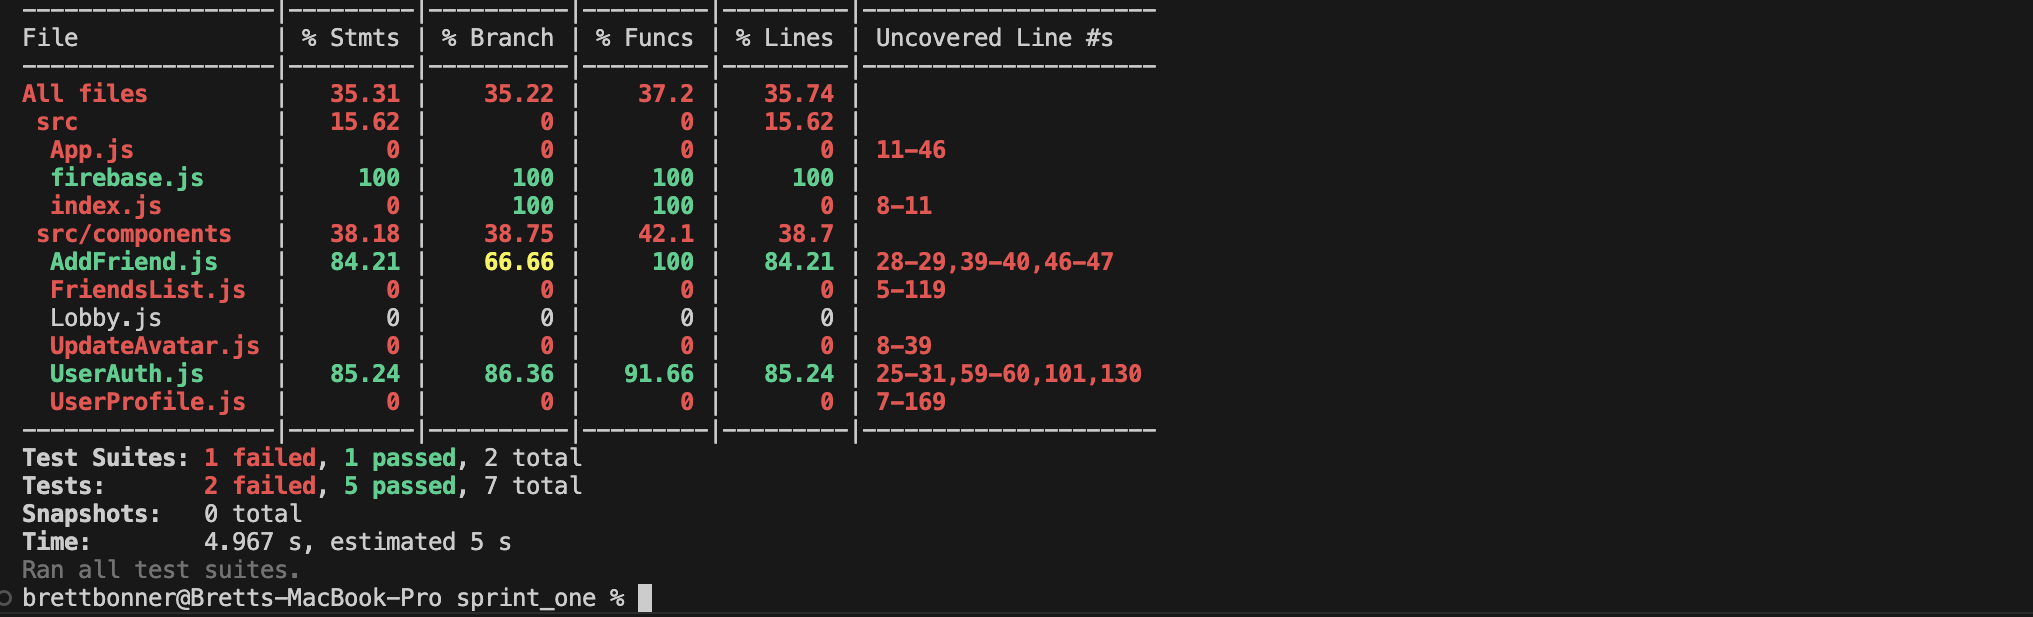
\includegraphics[width=1\linewidth]{figures/Testing-2.png}
    \caption{Sprint 1 Testing Output}
    \label{fig:enter-label}
\end{figure}

    We chose Jest as a testing framework. We attempted to do unit testing for branch and statement coverage, however, we struggled with connecting jest with our react components. We managed to get some of our code tested as shown in firebase.js, AddFriend.js, and UserAuth.js. For our next sprint we plan on solving the issue with testing with a spike to ensure we meet the specified requirements. 


 

\begin{table}[h]
\centering
No story changes or slices during this sprint.

\caption{Sprint 1 Story Distribution and Point Tracking}
\begin{tabular}{|p{3cm}|p{6cm}|c|c|}
\hline
\textbf{Team Member} & \textbf{Stories Attempted} & \textbf{Points Attempted} & \textbf{Status} \\
\hline
Ayoposi Olu & 
\begin{itemize}
    \item S4: Logout (1 pt)
    \item S5: Password (2 pts)
    \item S6: Update (1 pt)
\end{itemize} & 
4 & 
Completed \\
\hline
Jonathan Ramos & 
\begin{itemize}
    \item S7: Profile Avatar (2 pts)
    \item S8: Add Friend (2 pts)
    \item S9: Remove Friend (2 pts)
    \item S10: Show Friends (1 pt)
\end{itemize}& 
7 & 
Completed \\
\hline
Brett Bonner & 
\begin{itemize}
    \item S1: Create User (2 pts)
    \item S2: Guest Account (1 pt)
    \item S3: Login (1 pt)
\end{itemize} & 
4 & 
Completed \\
\hline
\multicolumn{4}{|c|}{} \\
\hline
\multicolumn{2}{|l|}{\textbf{Total Points Attempted}} & \multicolumn{2}{c|}{15} \\
\hline
\multicolumn{2}{|l|}{\textbf{Total Sprint Points (All Stories)}} & \multicolumn{2}{c|}{62} \\
\hline
\end{tabular}

\vspace{0.5cm}
\begin{center}
\small{Sprint 1 period from 10/17/2024 to 10/24/2024}
\end{center}
\end{table}

\begin{table}[h]
\centering
\caption{Team Velocity and Hours-per-Point Metrics}
\begin{tabular}{|l|c|c|c|}
\hline
\textbf{Team Member} & \textbf{Hours Worked} & \textbf{Story Points} & \textbf{Hours/Point} \\
\hline
Ayoposi Olu & 12 & 4 & 3 \\
\hline
Jonathan Ramos & 20 & 7 & 2.85 \\
\hline
Brett Bonner & 13 & 4 & 3.25 \\
\hline
\multicolumn{4}{|c|}{} \\
\hline
\multicolumn{2}{|l|}{\textbf{Team Totals}} & \textbf{14} & \textbf{2.857} \\
\hline
\end{tabular}

\begin{center}
\small{Sprint Velocity History}
\end{center}
\begin{tabular}{|l|c|c|c|c|}
\hline
\textbf{Sprint} & \textbf{Points Completed} & \textbf{Hours Worked} & \textbf{Hours/Point} & \textbf{Velocity} \\
\hline
Sprint 1 & 14 & 45 & 3 & 14 pts/sprint \\
\hline
\end{tabular}

\vspace{0.4cm}
\begin{center}
\small{Velocity = Points completed per sprint \\
Hours/Point = Total hours worked / Points completed}
\end{center}
\end{table}



\subsection{Sprint 2}

\subsubsection{Plan}
User Stories and Technical Tasks attempted in sprint 2 

Brett Bonner
\begin{itemize}
    \item S15: Private Chat (3 pts)
    \item S16: Review Chat (2 pts)
\end{itemize}


Ayoposi Olu

\begin{itemize}
    \item S17: Lobby (5 pts)
    \item Technical Task: Testing (2 pts)
\end{itemize}


Jonathan Ramos

\begin{itemize}
    \item S19: Table (5 pts)
    \item S21: Start Game (3 pts)
    \item S22: Bot (5 pts)
\end{itemize}

\subsubsection{Activities}
During this sprint we built on top of the working deliverable from sprint 1. This sprint began similarly to the last sprint, in which, we set up the database accordingly to handle chats and tables. We added two new collections to our Firestore component, properly names `chats' and `tables'. The chats collection creates a document for every chat that happens between two players. Each chat document has a single field which is an array of maps named messages. Each element in the array is a map containing three fields, senderID, text, and a timestamp. The tables collection creates a document for every table that is created between two players. Each table document has several fields, createdAt, createdBy, maxPlayers, playerIDs (array), players (array), and status. This document is filled appropriately when a player connects to the table. Once the host deals the cards, therefore starting the game, the players array is populated with a deck (array), the currentCard, and the score of each player. This document is essential for the driving the multiplayer game as it is vital that each user obtains the same information from the database in real-time. The tables collection is also necessary to populate our lobby with live tables as user's need to join or create a table to play online. 


\subsubsection{Retrospective}
During this sprint, we planned to complete about the same story points as sprint 1. \textbf{S19 Table}, was a challenging story to complete as it involved writing the entire game logic on the front-end and back-end. Additionally, S19 Table required players to connect and play the game in real-time. During the process of completing this user story, user stories \textbf{S21 Start Game} and \textbf{S22 Bot} were also completed. S22 was completed as the game logic was being developed, it was necessary to play with the computer to ensure the game logic was working properly on both the front-end and back-end. S22 Start Game was completed as when 2 players connected to a table, the host of the game needed to deal the cards and therefore start the game for both players. 

\subsubsection {Testing}
\begin{figure}[h]
    \centering
    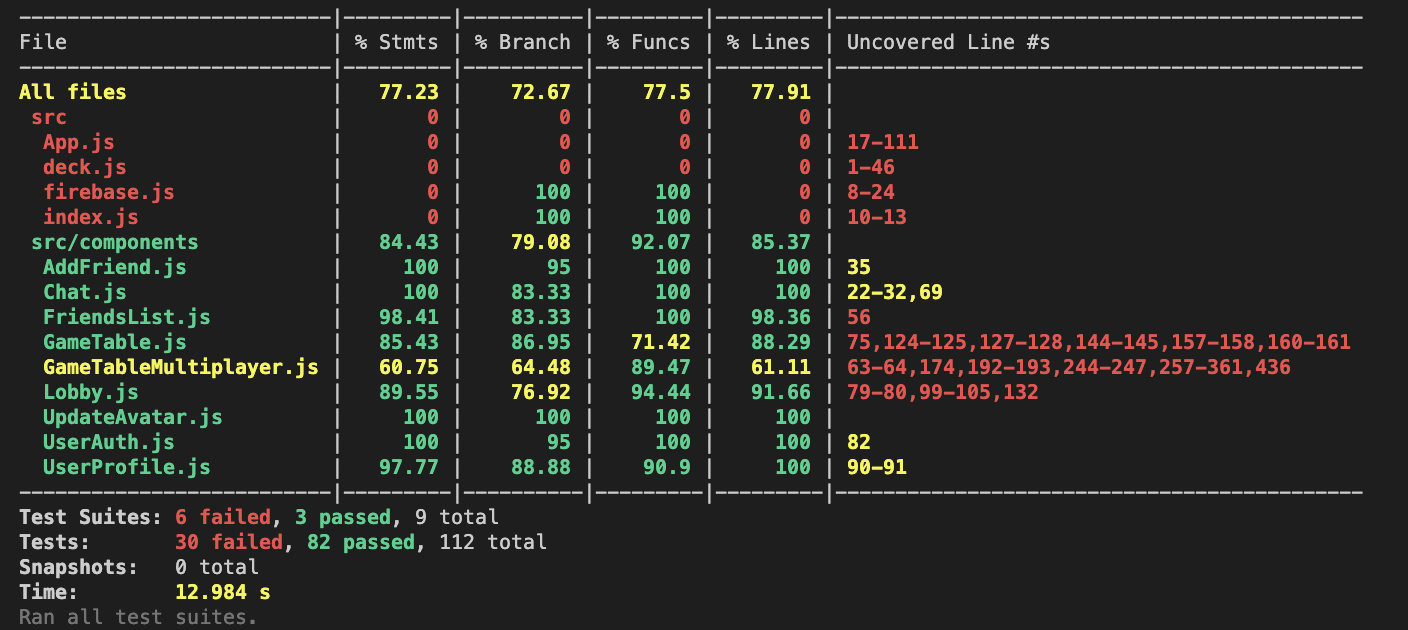
\includegraphics[width=1\linewidth]{figures/Testing.png}
    \caption{Sprint 2 Testing Output}
    \label{fig:enter-label}
\end{figure}

We improved on our testing coverage when compared to our testing coverage from sprint 1. Due to the challenges we faced with our testing framework and its dependencies, we used AI as a tool to help us clean up our testing environment and write tests based on the test cases we provided. We increased our statement coverage for all files to 77.23 percent and increased out branch coverage for all files to 72.67 percent. This is a significant increase when compared to our testing from sprint 1. 
     



\begin{table}[h]
\centering
No story changes or slices during this sprint.

\caption{Sprint 2 Story Distribution and Point Tracking}
\begin{tabular}{|p{3cm}|p{6cm}|c|c|}
\hline
\textbf{Team Member} & \textbf{Stories Attempted} & \textbf{Points Attempted} & \textbf{Status} \\
\hline
Ayoposi Olu & 
\begin{itemize}
    \item S17: Lobby (5 pts)
    \item Technical Task: Testing (2 pts)
\end{itemize} & 
7 & 
Completed \\
\hline
Jonathan Ramos & 
\begin{itemize}
    \item S19: Table (5 pts)
    \item S21: Start Game (3 pts)
    \item S22: Bot (5 pts)
\end{itemize}& 
13 & 
Completed \\
\hline
Brett Bonner & 
\begin{itemize}
    \item S15: Private Chat (3 pts)
    \item S16: Review Chat (2 pts)
\end{itemize} & 
5 & 
Completed \\
\hline
\multicolumn{4}{|c|}{} \\
\hline
\multicolumn{2}{|l|}{\textbf{Total Points Attempted}} & \multicolumn{2}{c|}{25} \\
\hline
\multicolumn{2}{|l|}{\textbf{Total Sprint Points (All Stories)}} & \multicolumn{2}{c|}{62} \\
\hline
\end{tabular}

\vspace{0.5cm}
\begin{center}
\small{Sprint period from 10/24/2024 to 11/07/2024}
\end{center}
\end{table}

\begin{table}[h]
\centering
\caption{Team Velocity and Hours-per-Point Metrics}
\begin{tabular}{|l|c|c|c|}
\hline
\textbf{Team Member} & \textbf{Hours Worked} & \textbf{Story Points} & \textbf{Hours/Point} \\
\hline
Ayoposi Olu & 22 & 7 & 3.14 \\
\hline
Jonathan Ramos & 35 & 13 & 2.69 \\
\hline
Brett Bonner & 15 & 5 & 3.0 \\
\hline
\multicolumn{4}{|c|}{} \\
\hline
\multicolumn{2}{|l|}{\textbf{Team Totals }} & \textbf{25} & \textbf{2.88} \\
\hline
\end{tabular}

\begin{center}
\small{Sprint Velocity History}
\end{center}
\begin{tabular}{|l|c|c|c|c|}
\hline
\textbf{Sprint} & \textbf{Points Completed} & \textbf{Hours Worked} & \textbf{Hours/Point} & \textbf{Velocity} \\
\hline
Sprint 2 & 25 & 72 & 2.88 & 19.5 pts/sprint \\
\hline
\end{tabular}

\vspace{0.5cm}
\begin{center}
\small{Velocity = Points completed per sprint \\
Hours/Point = Total hours worked / Points completed}
\end{center}
\end{table}


\subsection{Sprint 3}

\subsubsection{Plan}
User Stories and Technical Tasks attempted in sprint 3

Brett Bonner
\begin{itemize}
    \item S12: Display Stats (1 pt)
    \item S23: Manage Users (1 pt)
    \item S25: Manage Ads (3 pts)
\end{itemize}


Ayoposi Olu

\begin{itemize}
    \item S27: Notifications (1 pt)
    \item S18: Tutorial (3 pts)
    \item S20: Currency (1 pt)
\end{itemize}


Jonathan Ramos

\begin{itemize}
    \item S19: Table (5 pts)
    \item S21: Start Game (3 pts)
    \item S22: Bot (5 pts)
\end{itemize}



\subsubsection{Activities}
During this sprint we focused on completing admin user stories as we had not completed any admin functionalities yet. S19 Table was placed on the backlog for additional work. During this sprint, the user interface for the game was updated to become more interactive for the user. Additionally, we improved the logic for War to handle back-to-back wars when playing with a bot. As for multiplayer, we improved the user interface to becomes more interactive for both players. During this sprint we encountered an issue with the multiplayer game in which the system would read from the database a significant amount more than it needed to. Due to the high number of reads, we reached the limits of our database and unfortunately lost time in waiting for our quota to clear. This issue was fixed during this sprint, the multiplayer component was updated to only read from the database when the status field is updated, this greatly reduced the number of reads, and therefore fixing the issue. However, due to this unforeseen event, the tie-breaker (war) for multiplayer does not follow the traditional rules of the game. Due to time constraints, our multiplayer game handles war by returning each card back to the player that placed it. Display Stats and Manage Ads were both attempted and completed, however Manage users was not completed during this sprint. 


\subsubsection{Retrospective}
\textbf{S19 Table}, remained a challenging story to complete. Due to the unforeseen obstacle we faced with our database, we lost several hours of time needed to work on fully completing all of the features of the game. We also ran into issues with testing \textbf{S22 Bot} as the game logic changed from sprint 2 to support back-to-back wars. The user interface was also significantly changed from sprint 2. These changes caused our previous tests to no longer work as they depended on the structure of our previous code. Similarly, \textbf{S19 Table} was also significantly changed from sprint 2 to sprint 3 to support a more interactive user interface as well as updating the game logic to support the updated interactivity. The development of a tutorial was necessary during this sprint as we needed a way to give users a smooth understanding of the card game. Additionally, a simple currency was implemented into the game to add stakes for each a table. Notifications were implemented during this sprint as a functionality for an admin user, in which only they can send and modify notifications that go out to all users. One of the ways we could have been more efficient was to complete the multiplayer game first and build the supporting features around it. The multiplayer part quickly became more difficult than it seemed at first which resulted in time lost waiting for the table component to be completed. 


\subsubsection {Testing}
\begin{figure}[h]
    \centering
    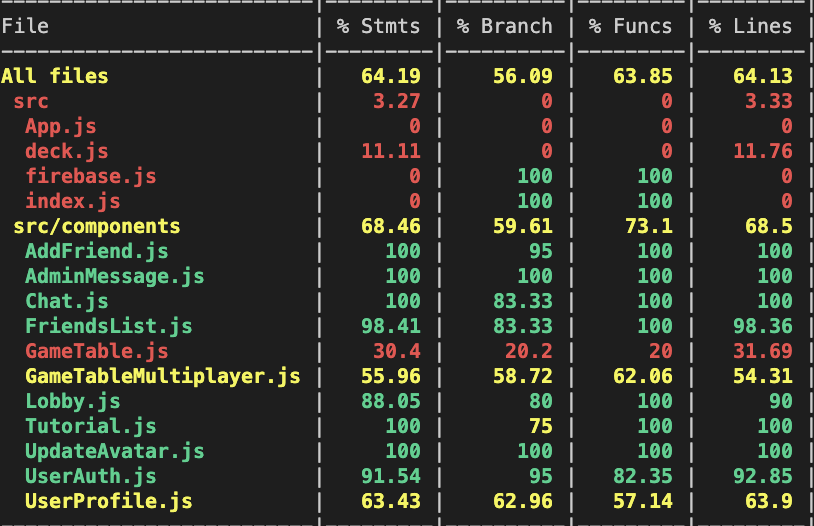
\includegraphics[width=1\linewidth]{figures/Testing sprint 3.png}  % dwb opmitted 'documentation/' ... what directory do you build this in? 
    \caption{Sprint 2 Testing Output}
    \label{fig:enter-label}
\end{figure}
Testing unfortunately decreased during this sprint due to the significant changes made to GameTable.js and GameTableMultiplayer.js. We also created tests for AdminMessage.js and Tutorial.js which were created during this sprint. 

     



\begin{table}[h]
\centering
No story changes or slices during this sprint.

\caption{Sprint 3 Story Distribution and Point Tracking}
\begin{tabular}{|p{3cm}|p{6cm}|c|c|}
\hline
\textbf{Team Member} & \textbf{Stories Attempted} & \textbf{Points Attempted} & \textbf{Status} \\
\hline
Ayoposi Olu & 
\begin{itemize}
    \item S27: Notifications (1 pt)
    \item S18: Tutorial (3 pts)
    \item S20: Currency (1 pt)
\end{itemize} & 
5 & 
Completed \\
\hline
Jonathan Ramos & 
\begin{itemize}
    \item S19: Table (5 pts)
    \item S21: Start Game (3 pts)
    \item S22: Bot (5 pts)
\end{itemize}& 
13 & 
Completed \\
\hline
Brett Bonner & 
\begin{itemize}
    \item S12: Display Stats (1 pt)
    \item S23: Manage Users (1 pt)
    \item S25: Manage Ads (3 pts)
\end{itemize} & 
5 & 
Completed \\
\hline
\multicolumn{4}{|c|}{} \\
\hline
\multicolumn{2}{|l|}{\textbf{Total Points Attempted}} & \multicolumn{2}{c|}{23} \\
\hline
\multicolumn{2}{|l|}{\textbf{Total Sprint Points (All Stories)}} & \multicolumn{2}{c|}{62} \\
\hline
\end{tabular}

\vspace{0.5cm}
\begin{center}
\small{Sprint period from 11/07/2024 to 11/21/2024}
\end{center}
\end{table}

\begin{table}[h]
\centering
\caption{Team Velocity and Hours-per-Point Metrics}
\begin{tabular}{|l|c|c|c|}
\hline
\textbf{Team Member} & \textbf{Hours Worked} & \textbf{Story Points} & \textbf{Hours/Point} \\
\hline
Ayoposi Olu & 16 & 5 & 3.2 \\
\hline
Jonathan Ramos & 25 & 13 & 1.92 \\
\hline
Brett Bonner & 13 & 5 & 2.6 \\
\hline
\multicolumn{4}{|c|}{} \\
\hline
\multicolumn{2}{|l|}{\textbf{Team Totals }} & \textbf{23} & \textbf{2.34} \\
\hline
\end{tabular}

\begin{center}
\small{Sprint Velocity History}
\end{center}
\begin{tabular}{|l|c|c|c|c|}
\hline
\textbf{Sprint} & \textbf{Points Completed} & \textbf{Hours Worked} & \textbf{Hours/Point} & \textbf{Velocity} \\
\hline
Sprint 1 & 14 & 45 & 3 & 14 pts/sprint \\
\hline
Sprint 2 & 25 & 72 & 2.88 & 19.5 pts/sprint \\
\hline
Sprint 3 & 23 & 54 & 2.34 & 20.33 pts/sprint \\
\hline
\end{tabular}

\vspace{0.5cm}
\begin{center}
\small{Velocity = Points completed per sprint \\
Hours/Point = Total hours worked / Points completed}
\end{center}
\end{table}

\section{System Architecture and Design}

%[[ Explain the architecture layering, perhaps include some UML, and mention the
%technologies used.

%Remember a picture is worth a thousand words! ]]

\subsection{Architecture}
We are planning on implementing a Model View Controller (MVC) architecture type for our game. It will be able to handle our in-game logic and how the user interacts with the game itself.
The Model typically will represent the game logic, deck and cards. The View will be responsible for representing the current state of the game to the user. Examples of this are displaying the players stats, profile and friends, having the ability to view output of cards/deck and showing tables in the lobby. We will be using a graphical feature to show this in our project. The Controller will handle user input for various commands like starting the game, ending the game, placing cards, party privacy and updating the players profile settings.

\subsection{Technologies}
Since we are developing a web-based version of the card game ``War", we have decided to use modern web technologies to ensure we have a responsive and scale-able application. Our front end will consist of common technologies used for web development, HTML, CSS, and Javascript. HTML will provide the basic structure of the web page, and CSS will allow us to style the page according to the theme specified by Cosmic Radiance. Javascript will handle game logic on the client side. Our front-end framework will be React.js as this will facilitate with updating the game-state without refreshing the page. React will also help with creating reusable components such as the cards themselves. 

Our back end will need to handle the game logic, player data, and real-time communication. Node.js will allow us to handle game logic outside of the browser. This will allow us the necessary means of handling requests such as determining winners. We will use a library Socket.io to handle real-time communication between multiple clients. 

To store our user data, game history, and player stats we will need persistent storage. We have chosen Firebase as our persistent storage due to its ease of use with real-time updates. It will also allow us to have a more flexible schema as SQL databases require relations among the tables created. Firebase also includes built-in authentication, supporting Google and Facebook sign in, as well as traditional email and password. Overall, Firebase supports our needs of real-time updates, scalability, security, and rapid development. 

\subsection{Persistent Storage}
Our database is composed of three main firebase components, Authentication, Firestore, and Storage. Each of these components is responsible for storing different types of information for each user. The authentication component is responsible for storing user login information, in our application this is the email and password of every user. Importantly, the Authentication component hashes passwords with a built-in function which improves security for our users. The storage component is responsible for storing the profile images of every user. The profile picture uploaded by the user is saved to the storage component under `avatars/user.uid' in which the current user's id is used as the filename. The majority of our user's data will be saved in the Firestore component. The data will be organized as JSON documents which are then organized into collections. The user's information such as, username, friends, stats, and profile picture URL will be saved into a document appropriately titled as the `user.uid'. Each user will require their own document, and all user documents will be stored in the `users' collection. This structure is flexible, making it scale-able which is important for an online multiplayer game. Our NoSQL design ensures that we can continue adding more collections and documents as needed without restructuring the entire database.

\subsection{Coding Standards}
Our database naming scheme will consist of singular, lowercase names for collections (user, leaderboard). Each attribute within documents will use camelCase (userName, gameStats, gameID). Variables and functions in JavaScript should also be written in camelCase. 

We will format our code using two spaces for indentation. Brackets should be used on the same line for functions and other control statements. Inline commenting should be used only to explain complex logic. Multi line comments should be used to describe functions and classes. Additionally, all functions should be properly documented with a multi-line comment describing the purpose, parameters, and return value. 

Testing standards will consist of test-driven development. We will ensure proper functionality by ensuring that all code commits pass necessary code tests before merging. Code tests should handle correctness, edge cases, and performance. 

\subsection{UML Diagram}
\begin{figure}
    \centering
    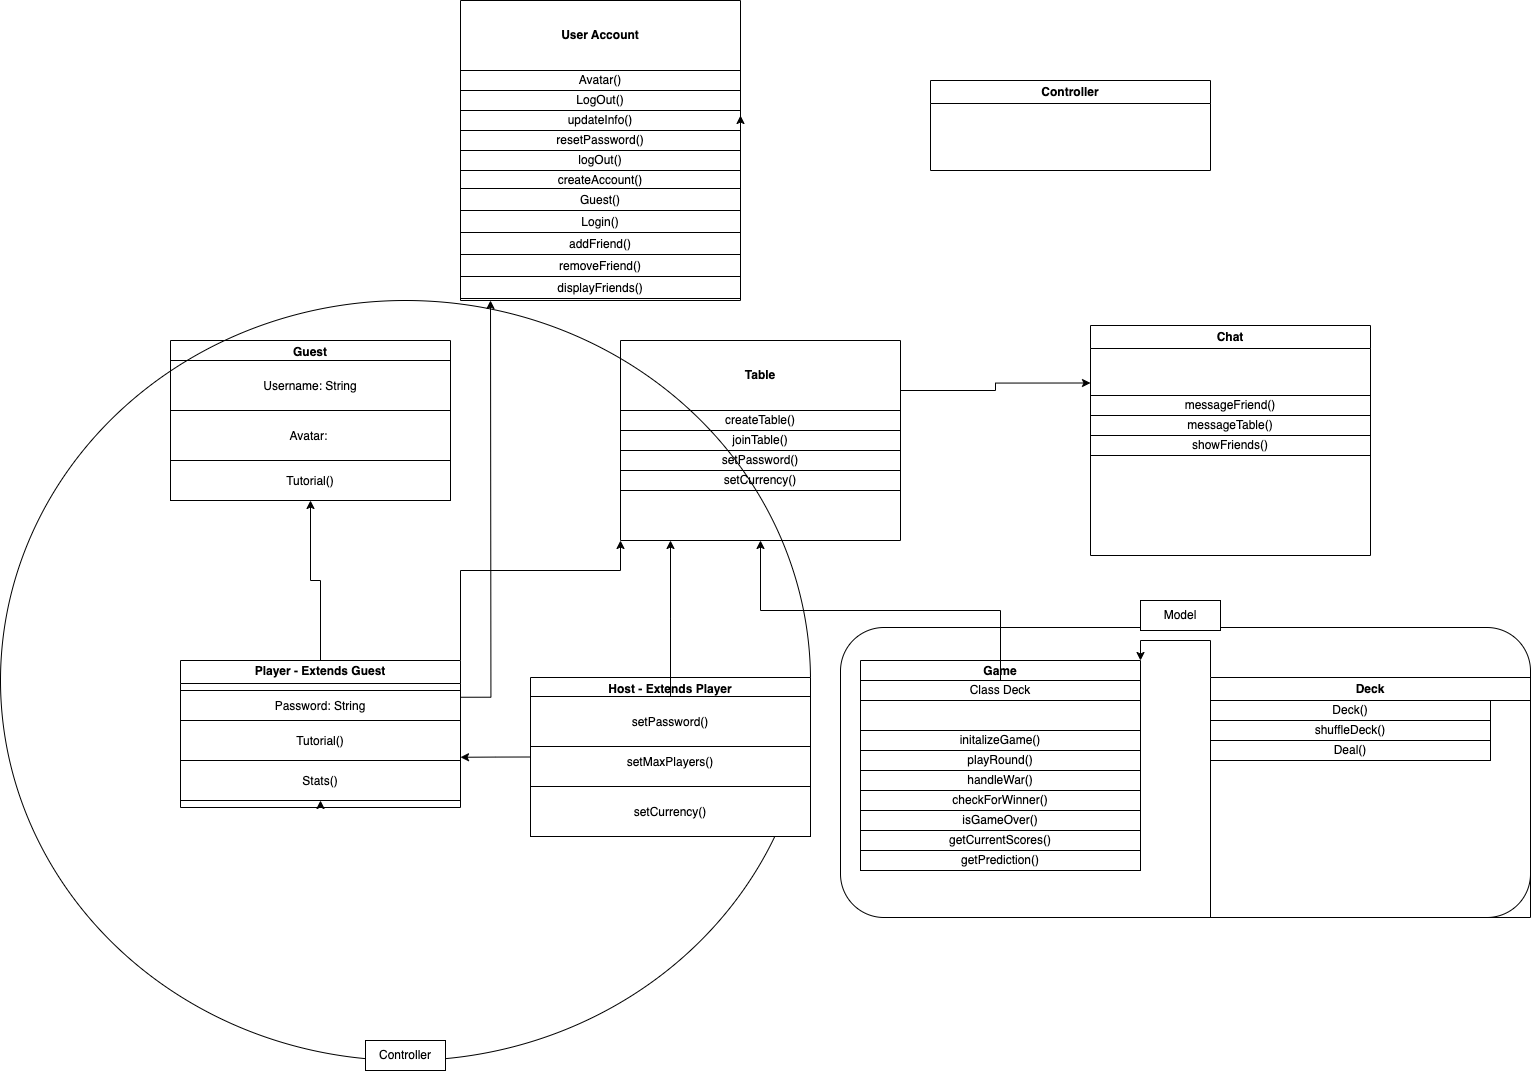
\includegraphics[width=1\linewidth]{figures/WarUML.png}
    \caption{UML diagram outlining the war card game for Cosmic Radiance}
    \label{fig:enter-label}
\end{figure}

\begin{figure}
    \centering
    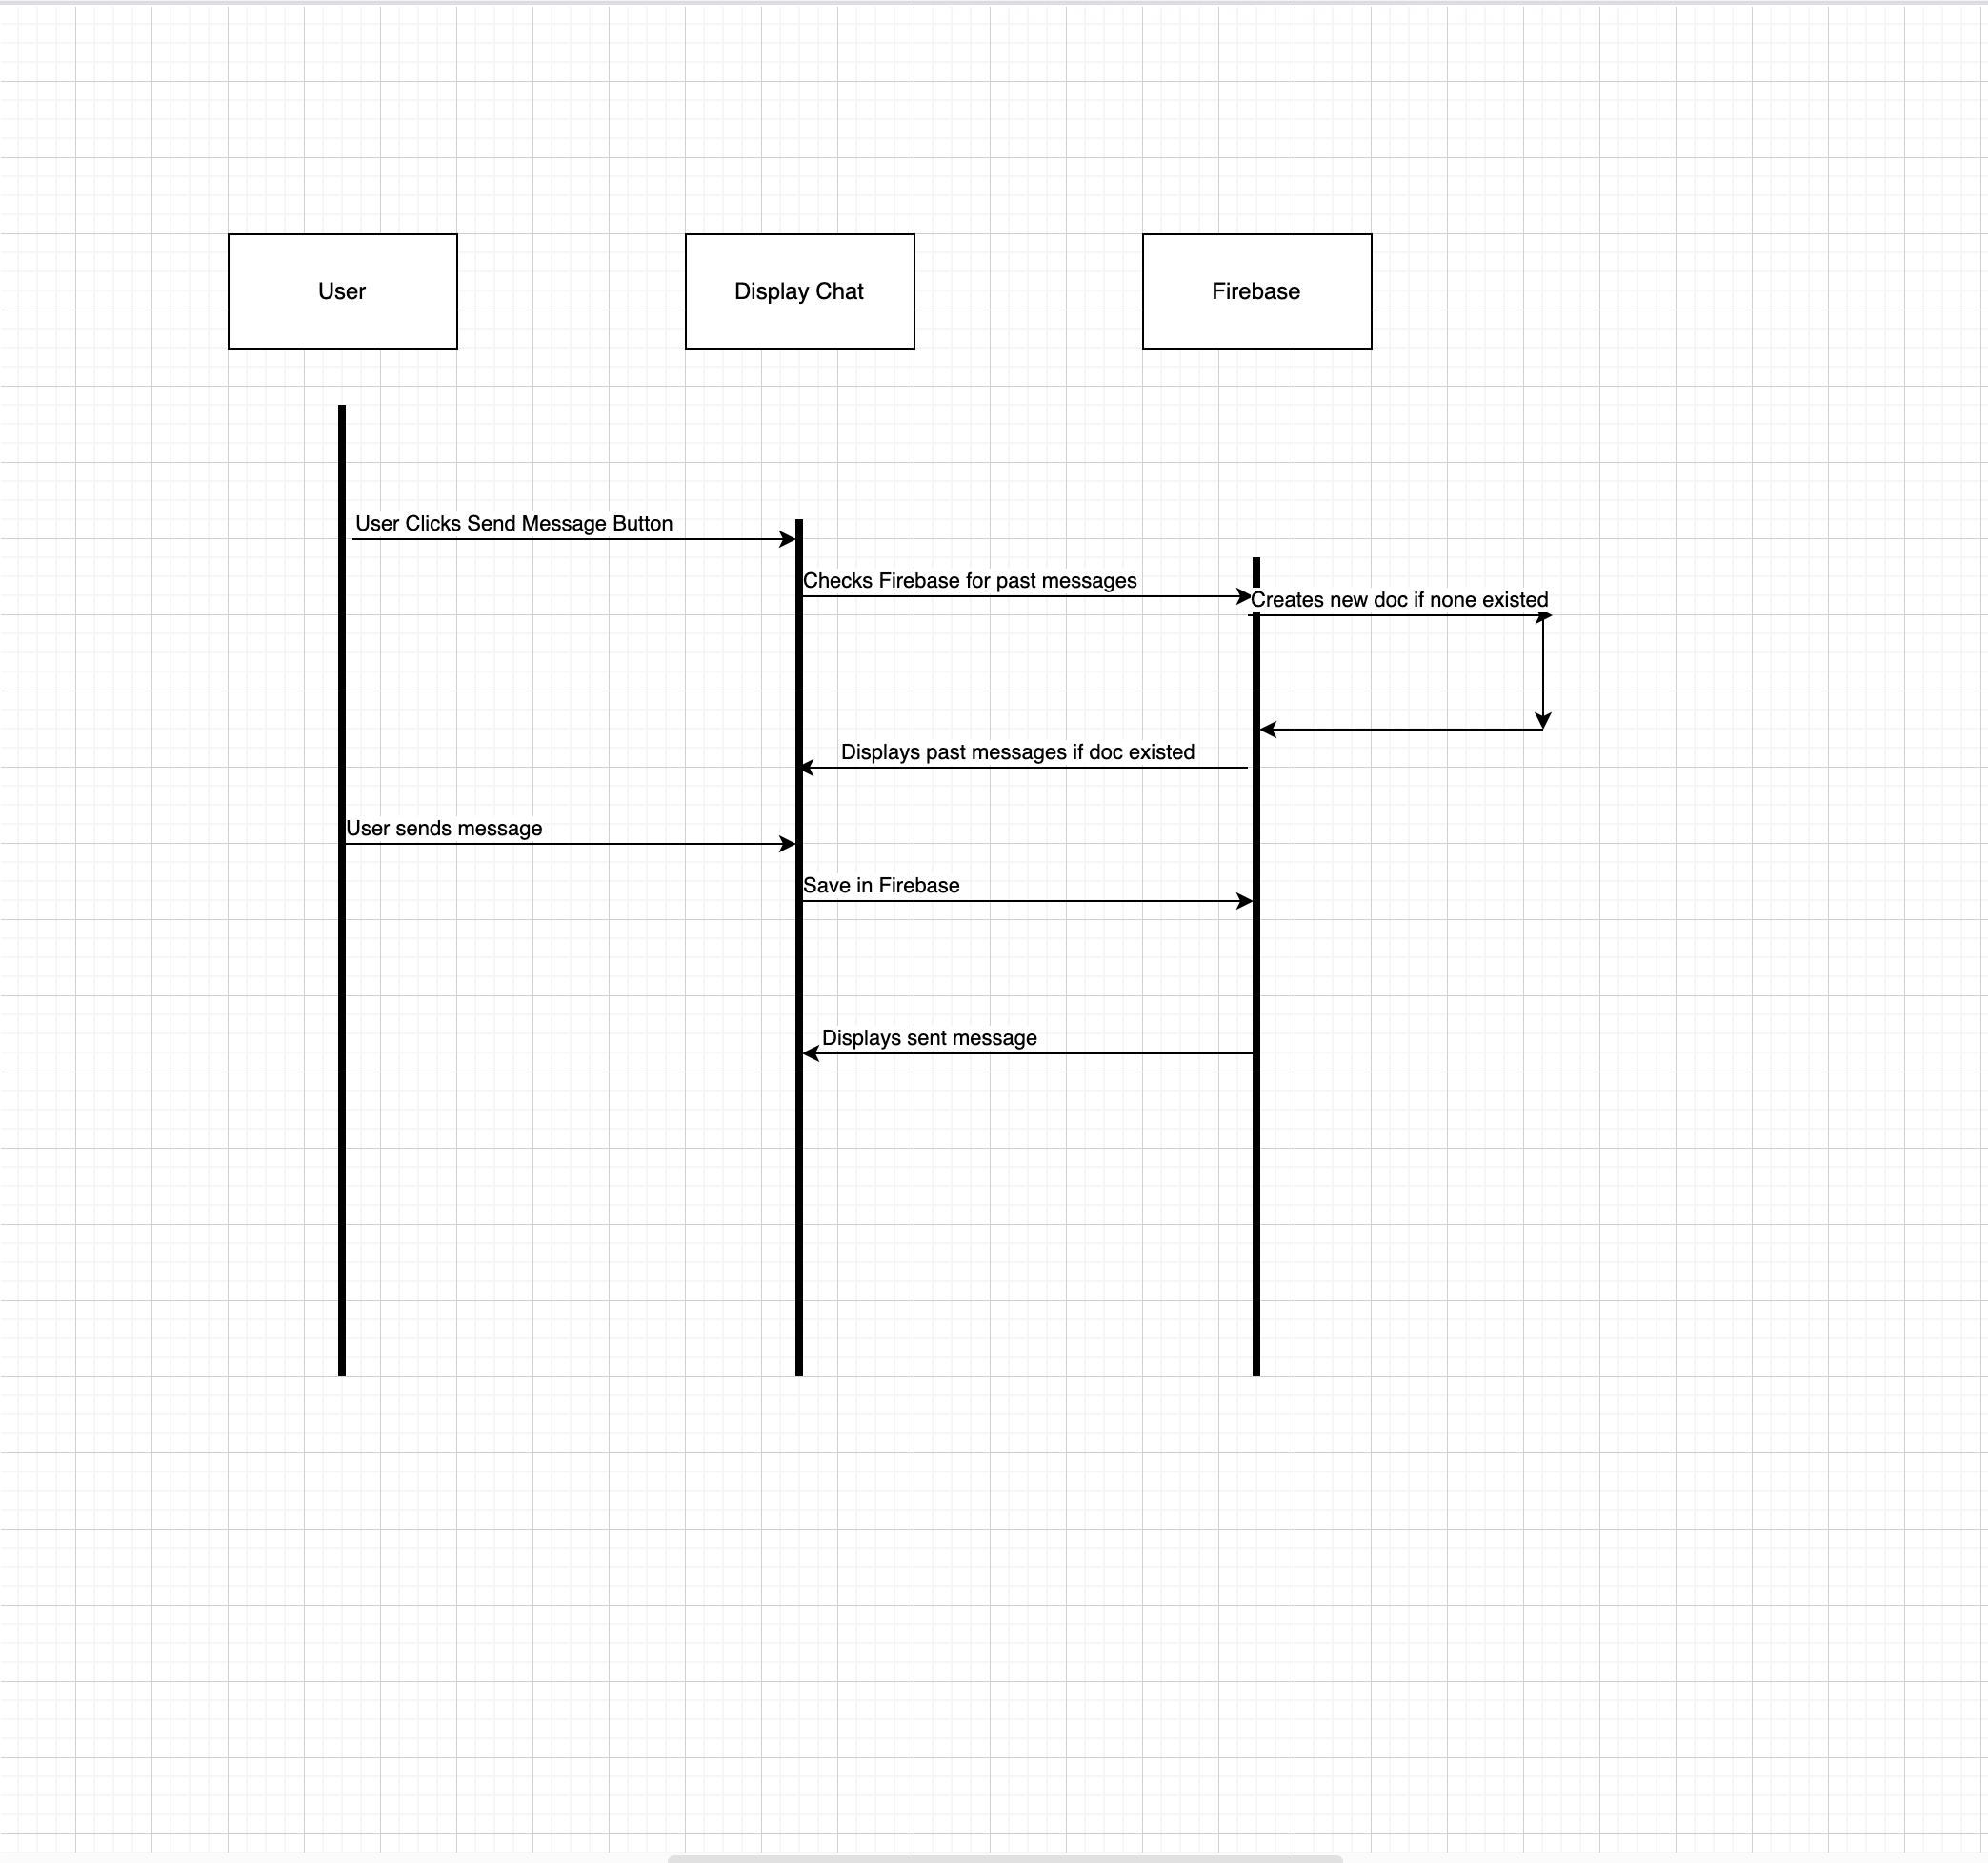
\includegraphics[width=1\linewidth]{figures/Sequence UML .png}
    % cd figures ; ln -s Sequence\ UML\ .png Sequence-UML.png 
    % who puts spaces in file names ;-)
    % \includegraphics[width=1\linewidth]{documentation/figures/sequence-UML.png}
    \caption{UML Sequence diagram for chat of War}
    \label{fig:enter-label}
\end{figure}

The system features a Host class that extends the player class, granting the host control over the table, including decisions on who can join. Additionally, a Game class manages the gameplay mechanics, ensuring that the rules of the game are followed. The User Account class manages all of the information of the User, from their password to avatar, to their friends. Lastly, a table class is made to allow users to join the table or create their own table.

\subsection {UI Mockups}
\begin{figure}
    \centering
    \includegraphics[width=1\linewidth]{figures/Welcome Page UI.png}
    \caption{The UI design for Cosmic Radiance web app's welcome screen features a space-themed layout with royal blue tones.}
    \label{fig:enter-label}
\end{figure}

\begin{figure}
    \centering
    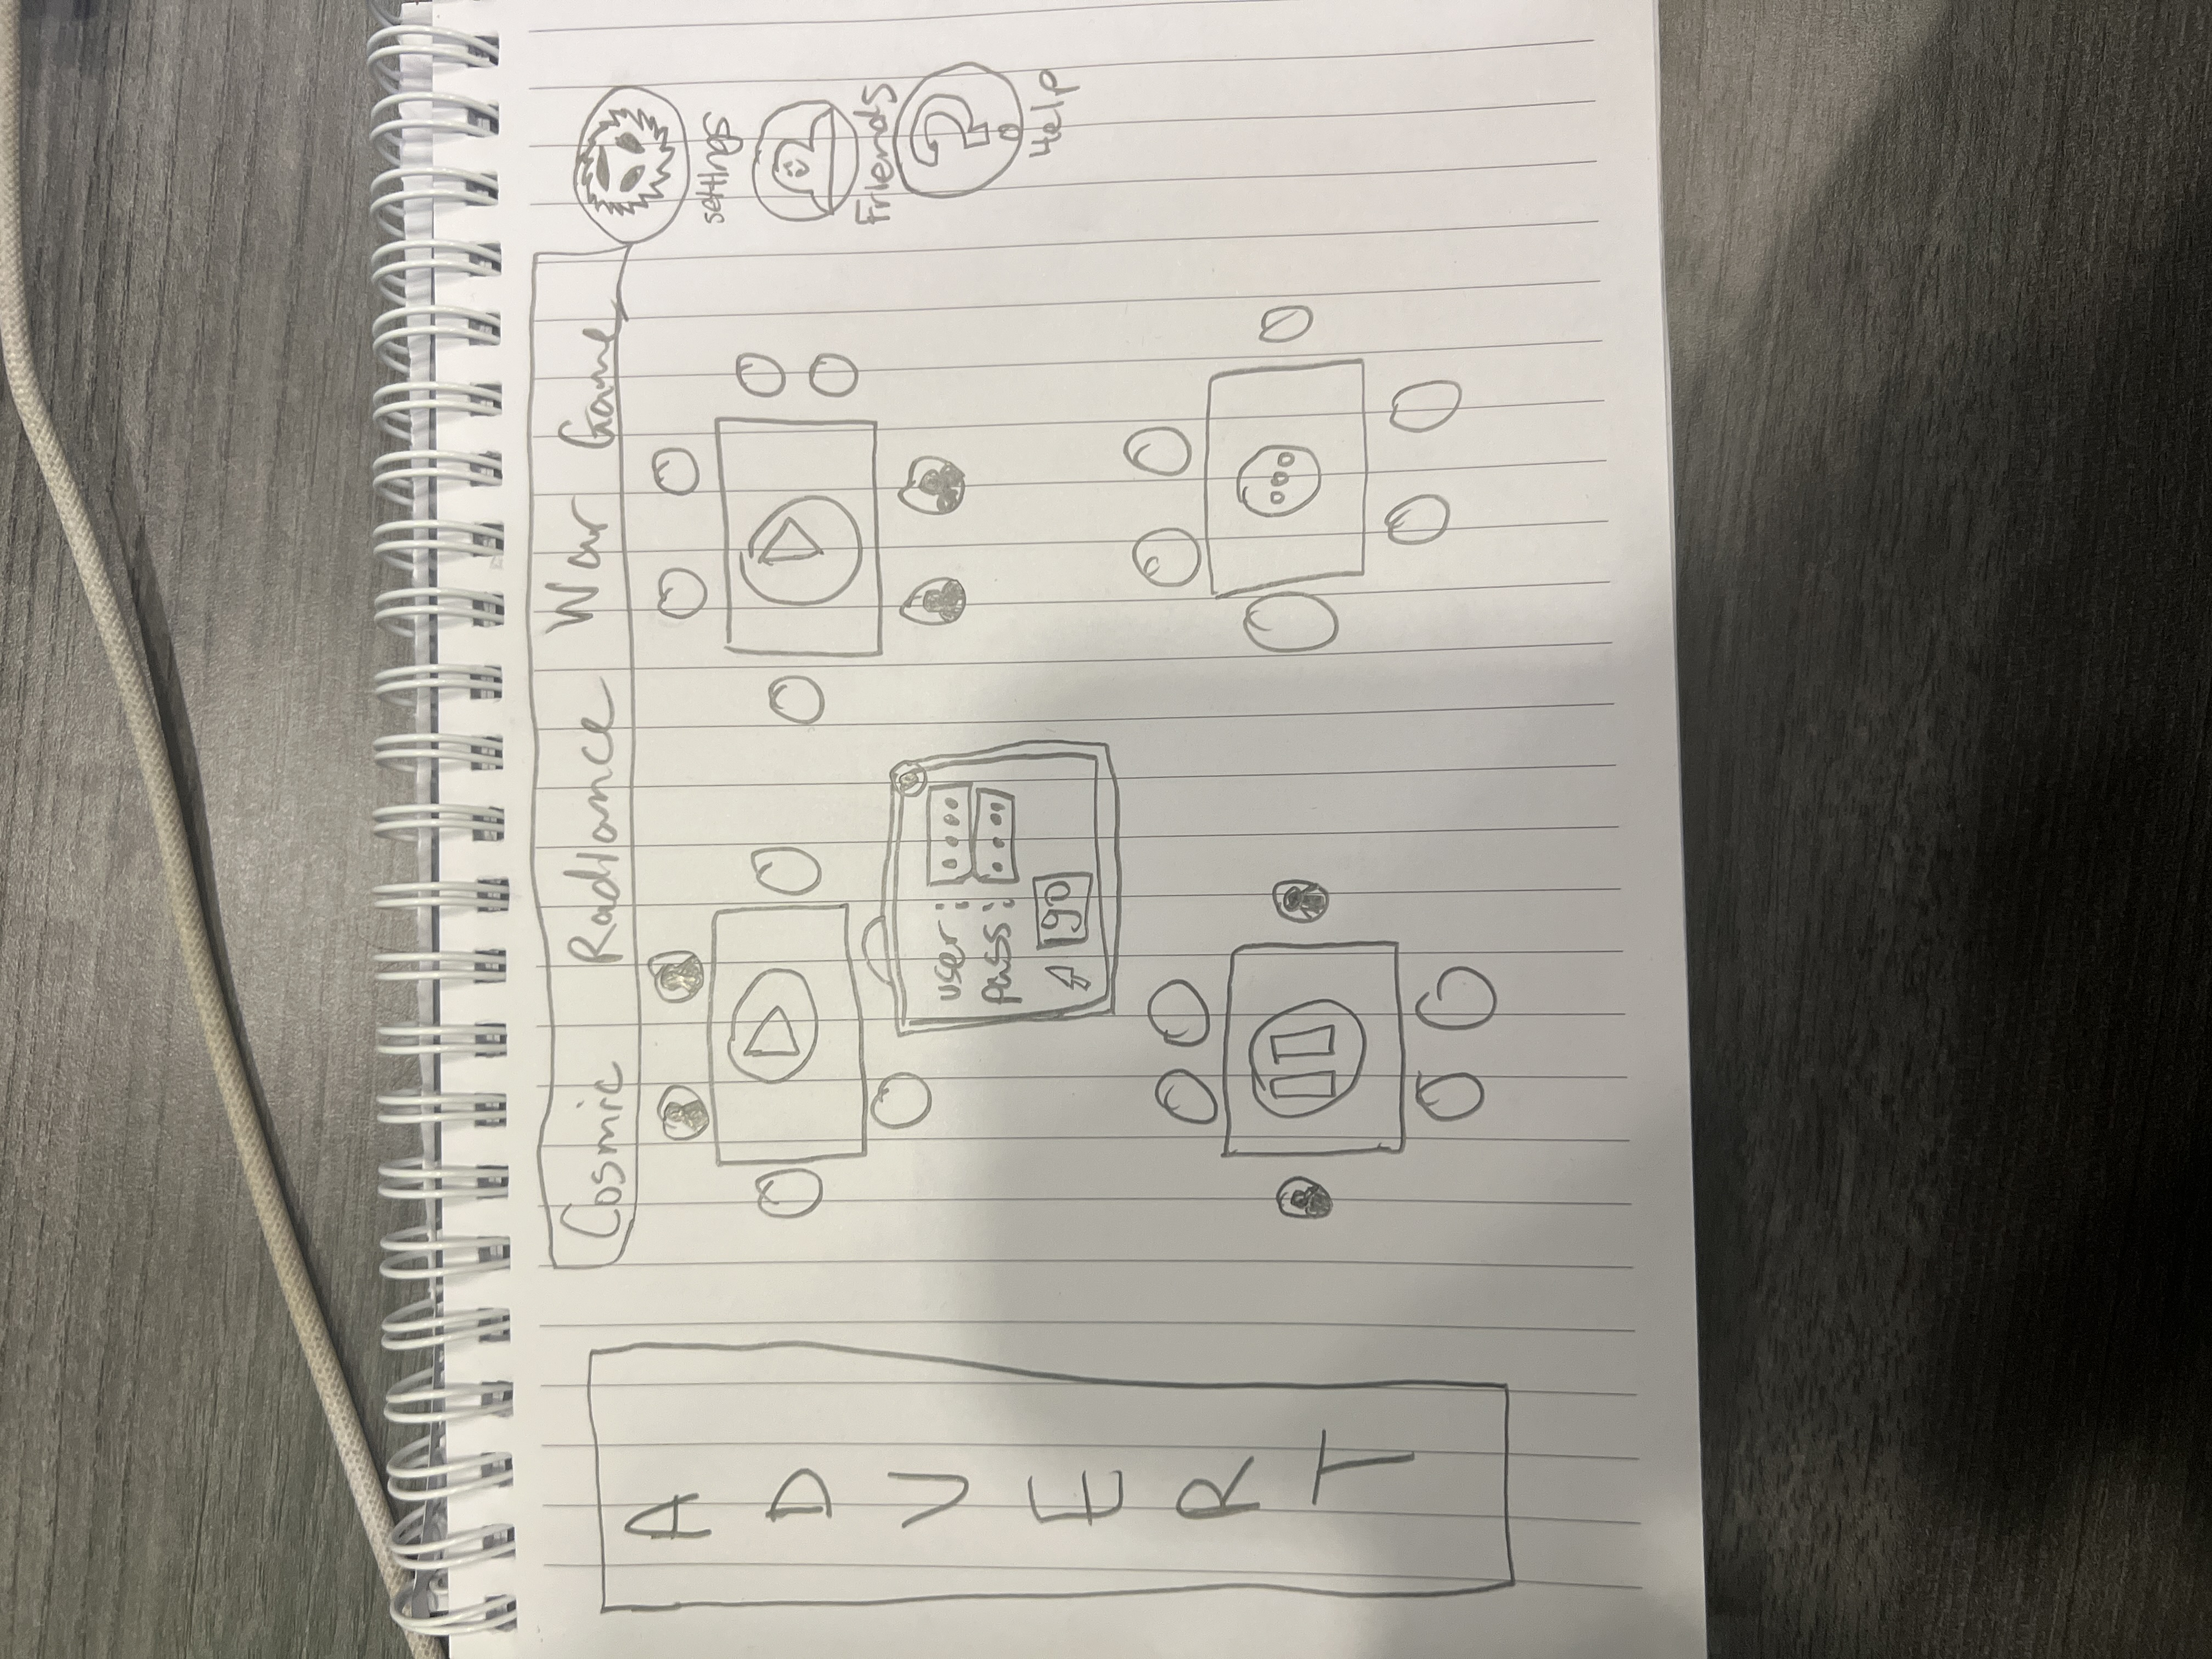
\includegraphics[width=1\linewidth]{figures/Lobby UI.jpeg}
    \caption{Lobby UI.}
    \label{fig:enter-label}
\end{figure}

\begin{figure}
    \centering
    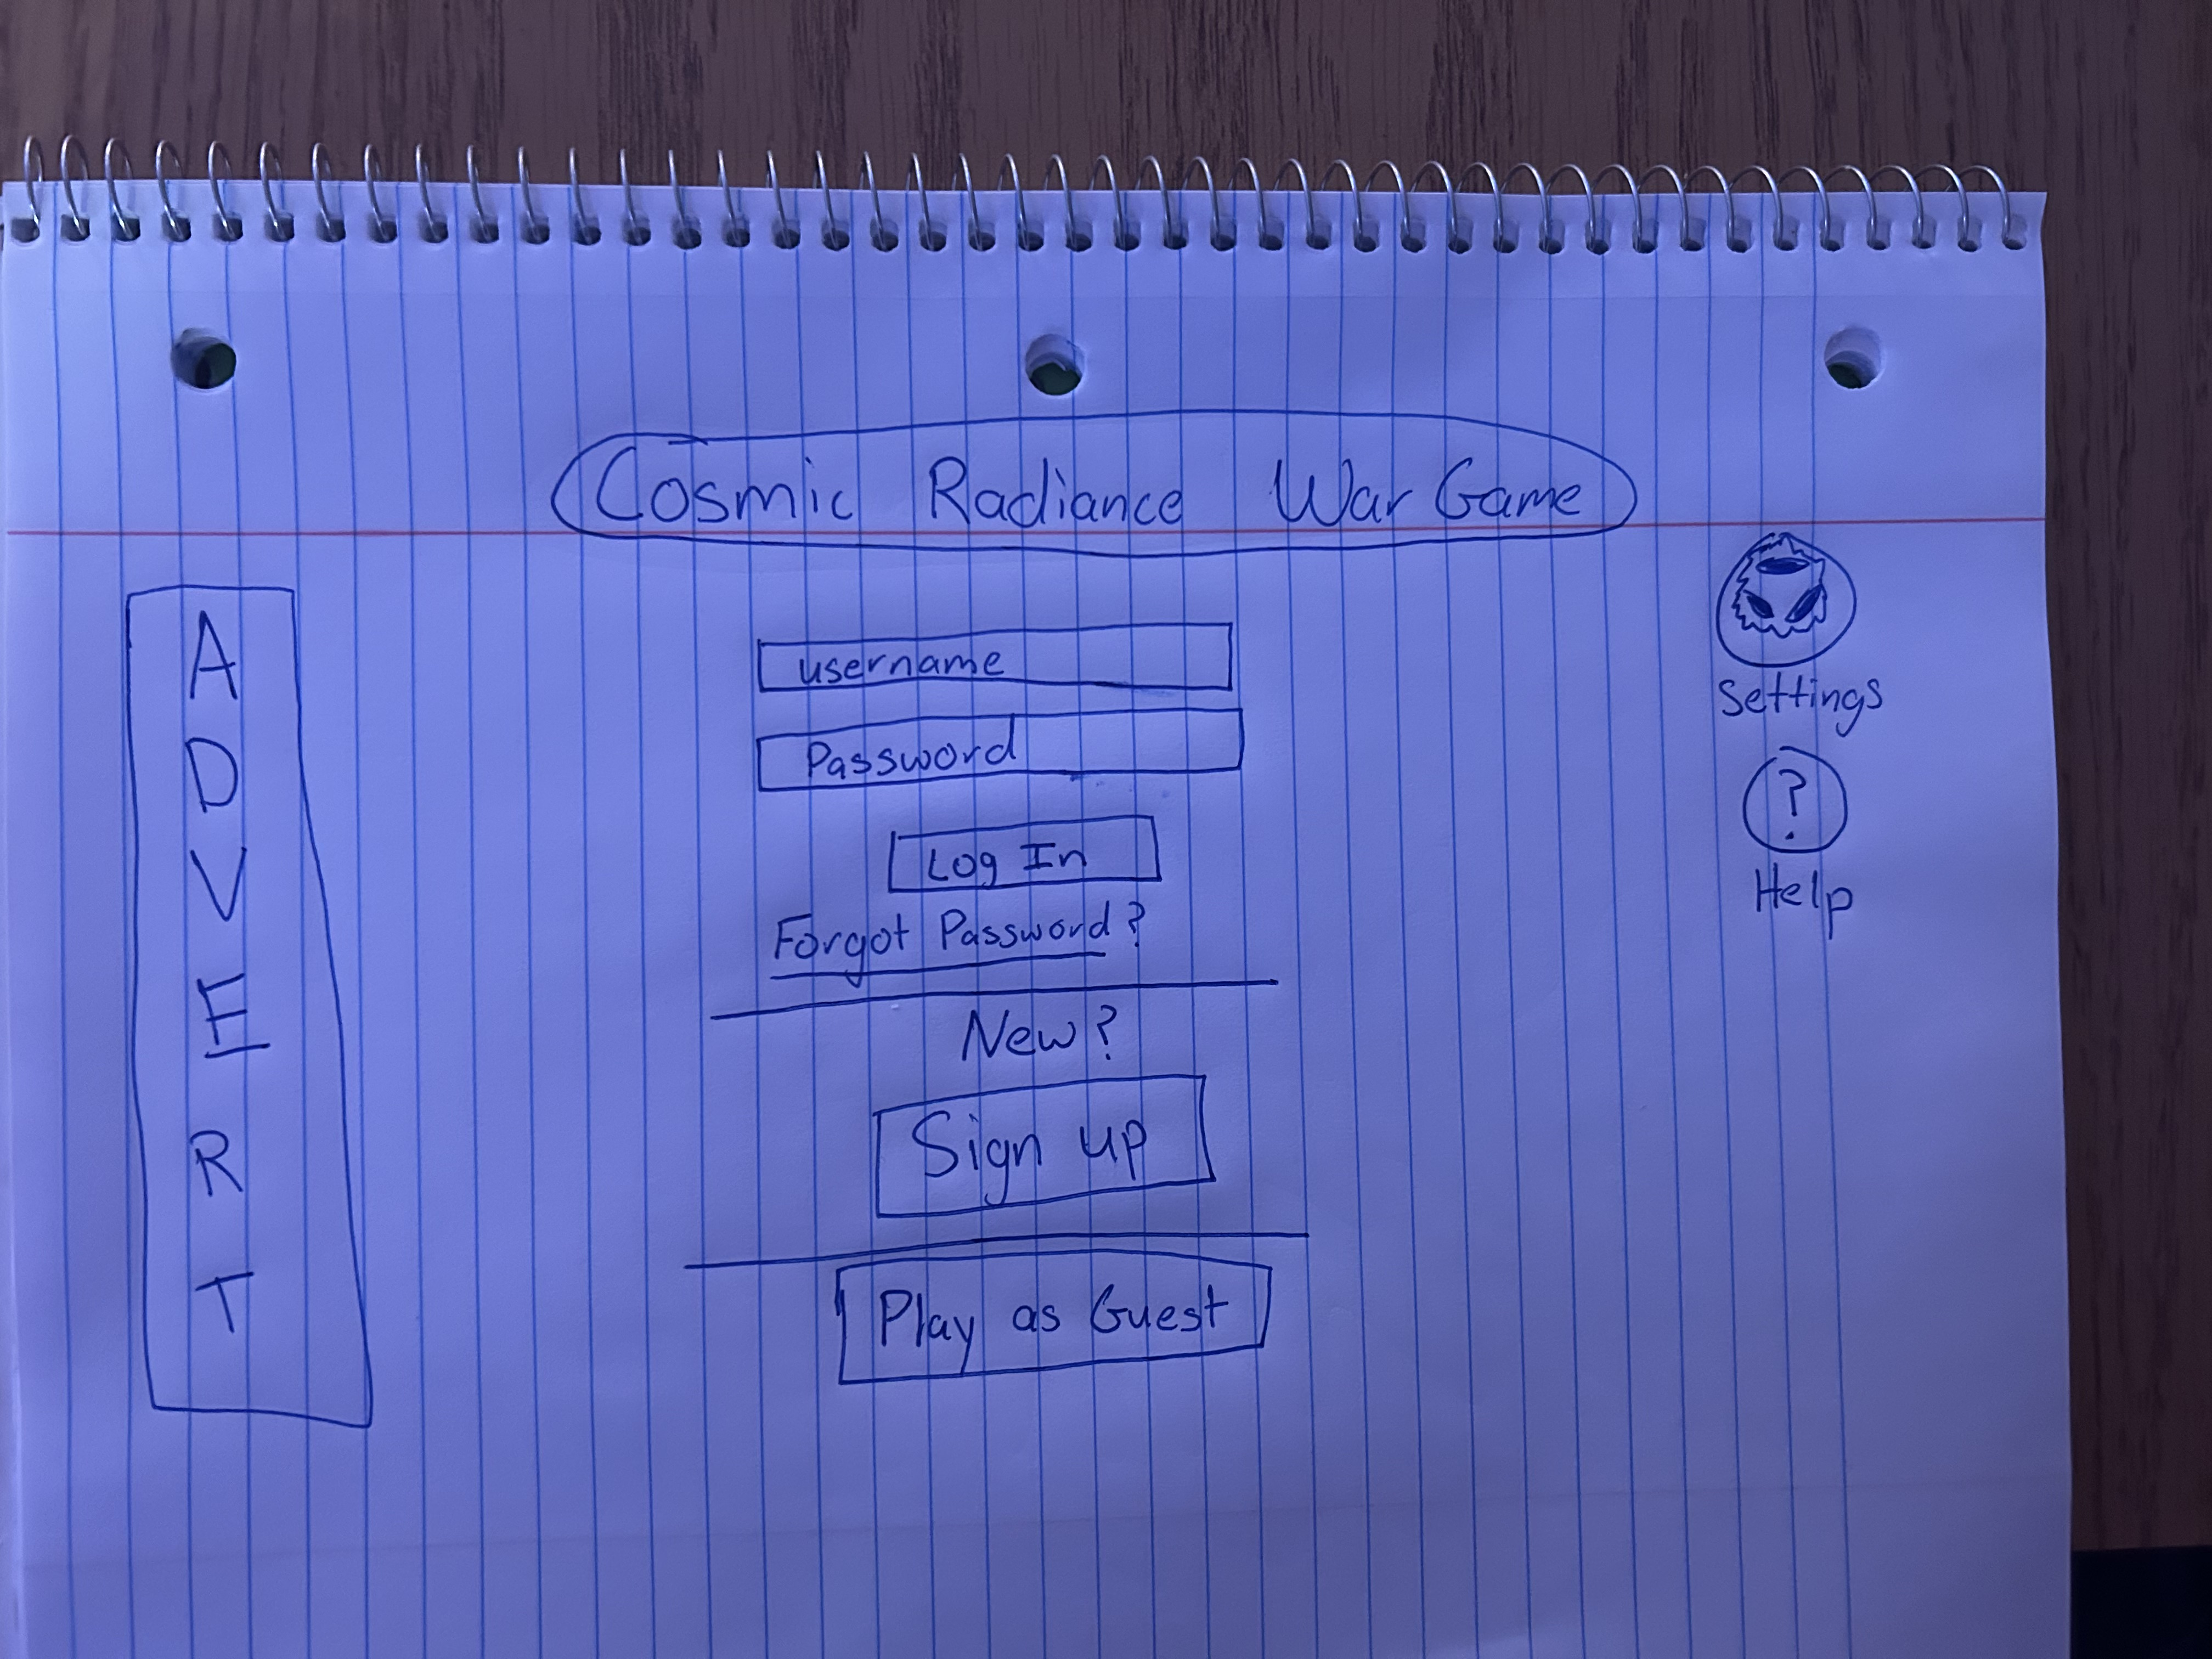
\includegraphics[width=1\linewidth]{figures/Login UI.jpeg}
    \caption{Login Screen for Cosmic Radiance War Game.}
    \label{fig:enter-label}
\end{figure}





\begin{minipage}{\textwidth}
\section {Testing}
\subsection{Internal Code Quality Analysis}
As shown in Table~\ref{tab:coverage-summary}, our project maintains a 68\% overall statement coverage, with 59.61\% branch coverage. The following points highlight our code quality achievements:
\begin{itemize}
    \item \textbf{Critical Path Coverage:} All critical business logic paths maintain coverage above 80\%.
    \item \textbf{Team Contribution:} Coverage responsibility is distributed across team members (Table~\ref{tab:member-coverage}).
\end{itemize}

\subsection{Areas for Improvement}
While our coverage metrics indicate strong testing practices, we've identified the following areas for enhancement:
\begin{itemize}
    \item GameTable.js requires additional edge case testing, currently at only 20.20\% branch coverage
    \item Integration test coverage for GameTableMultiplayer.js could be expanded
    \item Mock coverage for external dependencies in UserProfile.js could be improved
\end{itemize}

\vspace{1em}
\begin{center}
\captionof {Overall Test Coverage Summary for Components}
\label{tab:coverage-summary}
\begin{tabular}{|l|c|}
\hline
\textbf{Metric} & \textbf{Coverage \%} \\
\hline
Statements & 68.00\% \\
Branches & 59.61\% \\
Functions & 73.10\% \\
Lines & 68.50\% \\
\hline
\end{tabular}

\vspace{1em}
\begin{tabular}{|l|c|p{6cm}|}
\hline
\textbf{Team Member} & \textbf{Coverage \%} & \textbf{Primary Components} \\
\hline
Jonathan & 76.95\% & AddFriend, Friendslist, UpdateAvatar, GameTable, GameTableMultiplayer \\
Brett & 97.18\% & AdminMessage, Chat, UserAuth \\
Ayo & 83.83\% & Lobby, Tutorial, UserProfile \\
\hline
\end{tabular}

\vspace{1em}
\small
\begin{tabular}{|l|c|c|c|c|}
\hline
\textbf{Component} & \textbf{Stmt\%} & \textbf{Branch\%} & \textbf{Func\%} & \textbf{Line\%} \\
\hline
AddFriend.js & 100.00 & 95.00 & 100.00 & 100.00 \\
AdminMessage.js & 100.00 & 100.00 & 100.00 & 100.00 \\
Chat.js & 100.00 & 83.33 & 100.00 & 100.00 \\
FriendsList.js & 98.41 & 83.33 & 100.00 & 98.36 \\
GameTable.js & 30.40 & 20.20 & 20.00 & 31.69 \\
GameTableMultiplayer.js & 55.96 & 58.72 & 62.06 & 54.31 \\
Lobby.js & 88.05 & 80.00 & 100.00 & 90.00 \\
Tutorial.js & 100.00 & 75.00 & 100.00 & 100.00 \\
UpdateAvatar.js & 100.00 & 100.00 & 100.00 & 100.00 \\
UserAuth.js & 91.54 & 95.00 & 82.35 & 92.85 \\
UserProfile.js & 63.43 & 62.96 & 57.14 & 63.90 \\
\hline
\end{tabular}
\end{center}
\end{minipage} 
\section{Persistent Storage}
Our database is composed of three main firebase components, Authentication, Firestore, and Storage. Each of these components is responsible for storing different types of information for each user. The authentication component is responsible for storing user login information, in our application this is the email and password of every user. Importantly, the Authentication component hashes passwords with a built-in function which improves security for our users. The storage component is responsible for storing the profile images of every user. The profile picture uploaded by the user is saved to the storage component under `avatars/user.uid' in which the current user's id is used as the filename. The majority of our user's data will be saved in the Firestore component. The data will be organized as JSON documents which are then organized into collections. The user's information such as, username, friends, stats, and profile picture URL will be saved into a document appropriately titled as the `user.uid'. Each user will require their own document, and all user documents will be stored in the `users' collection. This structure is flexible, making it scale-able which is important for an online multiplayer game. Our NoSQL design ensures that we can continue adding more collections and documents as needed without restructuring the entire database.

\section{Reflections on the Project}
\section{AI Impact}

\subsection{Ayo}
My experience using AI/LLMs was a educational experience. Upon encountering our first roadblock. My team decided to assign me the technical task of learning how testing works. At first, understanding it myself was quite a challenege as I was completely unfamiliar with the Javascript testing framwork. The LLM was able to break up the code i produced and give me sample test cases I could use for testing. Another way LLMs helped me was in understanding how css components integrate into testing and the necessary field attributes that go into the test file and running it in the console.

\subsection{Jonathan}
I chose to limit my use of AI/LLMs for this application as often the code it produced did not work smoothly due to the complexity of the project. When developing the game logic, using AI/LLMs became more of a hassle than a tool as I spent more time debugging than actually programming. However, AI/LLMs were particularly useful for CSS, as my knowledge of CSS was quite limited before the project was started. 

\subsection{Brett}
Throughout the project, I found myself using AI quite a bit for various reasons. Whenever I ran into bugs or when things weren’t working as expected, I’d turn to AI for debugging help. AI was also a big help when it came to styling with css. However, getting AI to understand exactly what I wanted design-wise was a little tricky. I often had to go back and forth with multiple prompts to narrow down what I wanted. Besides that, anytime I had questions while coding, I would use AI for quick answers. Overall, AI was an extremely valuable tool throughout the project and made the overall process much smoother.

%\section{References}
%\bibliographystyle{plain}
%\bibliography{references}

%
\section{\LaTeX ``Tutorial''}

OMIT this section in production, but here is some sample \LaTeX~to munch on.

Use the table environment to include tables.
Be sure to keep the label and caption below the tabular!

Setting up tables can be annoying. You can also set it up in excel and then
copy it into \textsf{https://www.tablesgenerator.com} to generate the latex. 



\begin{table}[h!]
    \centering
    \begin{tabular}{|c|c|c|c|c|}
    \hline
      Risk   & Impact & Priority  & Overall Rating  & Mitigation \\
         &  &  &  & \\\hline
         &  &  &  & \\\hline
         &  &  &  & \\\hline
    \end{tabular}
    \caption{Risks to the software.}
    \label{tab:risks}
\end{table}

Table~\ref{tab:risks} overviews the risk relevant to our project.


Use the figure environment to include images such as \textsf{.png} in your latex document. \\

\begin{figure}[!bh]
\centering

\includegraphics[width=0.33\textwidth]{figures/sb.png} \\
\caption{Class Diagram for Sponge Bob's Best Christmas Ever.}
\label{fig:class}
\end{figure}

Figure~\ref{fig:class} shows the high-level class diagram.


\begin{figure}[!bht]
\begin{lstlisting}[language=Java]
public static void main(String [] args)
{
  System.out.println("Hello World!");
}
\end{lstlisting}
\caption{Hello Example.}
\label{fig:hello}
\end{figure}

Figure~\ref{fig:hello} shows the code used to print hello.
\textbf{Note that you writeup should include code sparingly.
The details of the code are not its focus.}



\end{document}

